\graphicspath{{/Users/brunomedina/Dropbox/Tesis-Egobets/egobets-notas/resources/}}

\chapter{Sistematización de las apuestas}
\label{chap:mate}

% En este capítulo se presentan, sin entrar al detalle técnico, los resultados comprobables de las teorías que proporcionan las probabilidades de los resultados de los partidos y las predicciones de sus resultados. De igual manera se destaca la importancia de un sistema de reservas para optimizar las tasas de crecimiento de la cantidad de dinero dedicada a las apuestas. Finalmente se retoman estos conceptos y se detalla el algoritmo que utiliza Egobets para la generación de las recomendaciones de apuestas.

En este capítulo se detallan las variables y los pasos que tiene el método utilizado por el sistema de Egobets para proveer a sus usuarios de una asesoría de apuestas personalizada. En la primera parte del capítulo, a modo de introducción, se discutirá si es posible modelar de manera matemática un partido de futbol con la finalidad de predecir su resultado. Además, en esta misma sección se explica como el afamado criterio de Kelly introduce la noción de un sistema de reservas y busca optimizar la ganancia esperada en función de restringir la fracción de dinero a invertir en cada partido.

\section{Antecendetes y evidencia a favor}
\label{sec:evidencia}

Esta tesis no busca predecir los resultados de los partidos de futbol, sin embargo es importante mostrar que esto se puede lograr y que más de algún autor ha encontrado maneras teóricas eficientes de hacerlo. De igual manera, se explica (sin entrar a detalle) uno de los modelos más utilizados en este ámbito: la Poisson bivariada. Esto ayuda al lector a comprender cuales son las variables que parecen afectar más los resultados y le permite tener una mejor noción de lo que puede ser una buena apuesta.

Después de exhibir el modelo, se presentan dos ejemplos concretos de estrategias de apuestas: la estrategia simple (e intuitiva) y la estrategia de Kelly. En particular, Kelly le da al problema un paradigma financiero y abre el camino a buscar apuestas que no arriesguen todo el capital del jugador. Esta idea será retomada en la siguiente sección para el sistema de reservas.

\subsection{Modelar un partido de futbol}
\label{subsec:modelo}


% El tema central de esta tesis no es la predicción de resultados de futbol principal si no la generación automatizada de recomendaciones de apuestas, por este motivo y para evitar cuestiones de plagios del modelo predictivo de Egobets, en este apartado no se entrarán en los detalles de la implementación, solamente se mostrarán las teorías los modelos matemáticos prácticos que permiten predecir los resultados de los partidos de futbol sobre los que se basa Egobets. Los resultados de los estudios analizados en esta sección son suficientes para evidenciar la existencia de un conjunto de probabilidades y resultados estimados que permitan desarrollar una estrategia de apuestas capaz de generar un valor esperado positivo.
%


Dixon y Coles (1997) \cite{dixon1997modelling} en su contribución, mencionan algunas propiedades deseables en un modelo de futbol:
\begin{itemize}
	\item Se deben considerar las habilidades de ambos equipos en un partido.
	\item Se debe dar lugar a la ventaja observada que tienen los equipos al jugar en casa.
	\item La medida más razonable de la habilidad de un equipo debe basarse en el desempeño de sus últimos juegos.
	\item La habilidad de un equipo, por la naturaleza del futbol, se comprende como la composición de la habilidad de ataque (anotar goles) y la habilidad de defensa (no recibir goles).
	\item Al presentar el desempeño de un equipo en sus recientes resultados, se deberá tomar en cuenta la habilidad de los equipos contra los cuales ha jugado.
\end{itemize}


 \subsubsection{Modelo de Poisson bivariada}
 \label{subsubsec:bivariate-poisson}

Koopman y Lit (2013) \cite{koopman2013dynamic} proponen el siguiente modelado de los partidos de futbol.
\begin{itemize}

	\item Supóngase que se tienen $J$ equipos en una liga donde cada semana juegan todos los equipos.

	\item Los equipos juegan dos veces contra todos los demás equipos, una vez de visitante y otra de local.
	\item Tómese el par $(X_{it},Y_{jt})$ como la cantidad de goles del partido. 
	\begin{itemize}
	
		\item $X_{it}$ es el número no negativo de goles anotados por el equipo local $i$ en la semana $t$.
		\item $Y_{jt}$ corresponde al número de goles anotados por el equipo visitante $j$ en esa misma semana $t$.
	\end{itemize}
		
		Para $i\neq j = 1, ...,J$ y $t=1,...,n$, con $n$ la cantida de semanas con partidos jugados (es decir que tienen datos).
\end{itemize}

\paragraph{Distribución Poisson Bivariada} % (fold)
\label{par:distribucion_poisson_bivariada}
Cada par de cuentas $(X,Y) = (X_{it},Y_{jt})$ se genera de una distribución Poisson bivariada con la siguiente función de masa de probabilidad:
 
 \[p(X,Y;\lambda_x,\lambda_y,\gamma) =\]
  \[e^{(-\lambda_x-\lambda_y-\gamma)}\frac{\lambda^X_x}{X!}\frac{\lambda^Y_y}{Y!}\sum_{k=0}^{min(X,Y)}\left(\frac{X}{k}\right)\left(\frac{Y}{k}\right)k!\left(\frac{\gamma}{\lambda_x\lambda_y}\right)^k \]

 para $X = X_{it}$ y $Y = Y_{it}$.
 Con $\lambda_x$ y $\lambda_y$ coeficientes que reflejan la intensidad de goleo para $X$ (equipo) y $Y$ (visitante) respectivamente en la jornada $t$.
 Y con $\gamma$ siendo el coeficiente que mide la dependencia entre los goles anotados por el local y el visitante $(X,Y)$. 

 La notación corta se describe como\footnote{La definición que se presenta en este documento es propuesta por \cite{koopman2013dynamic}, sin embargo hay otras variantes de esta fórmula \cite{kocherlakota1992bivariate} y \cite{johnson1997discrete}}:
 \boldmath\[(X,Y) \sim BP(\lambda_x,\lambda_y,\gamma)\]\unboldmath 
 % paragraph distribucion_poisson_bivariada (end)
 

\paragraph{Valor Esperado, Varianza y Covarianza} % (fold)
\label{par:valor_esperado}
 \[E(X) = \mathrm{Var}(X) = \lambda_x + \gamma \text{, } E(X) = \mathrm{Var}(Y) = \lambda_y + \gamma\]
 
 \[\mathrm{Cov}(X,Y) = \gamma\]


 y el coeficiente de correlación entre $X$ y $Y$ está dado por:
 \[\rho = \frac{\gamma}{\sqrt{(\lambda_x+\gamma)(\lambda_y+\gamma)}}\]
 
% paragraph valor_esperado (end)




\subsubsection{Intuición detrás del modelo}
\label{subsubsec:intuicion}
 El resultado de restar los goles del local menos los del visitante $X-Y$ determina si el partido fue ganado, perdido o empatado por el equipo de casa\footnote{La variable $X-Y$ tiene una distribución de probabilidad discreta conocida como: Skellman y conlleva muchas propiedades descritas en Skellman (1946) \cite{skellam1946frequency}}. Esta noción de modelar los partidos en función de la cantidad de goles de cada equipo se retoma del artículo de Maher (1982) \cite{maher1982modelling}, en el cual se narra que la posesión del balón origina la oportunidad de atacar y anotar un gol. La probabilidad de que un ataque resulte en gol puede ser pequeña, pero se debe recordar que son muchas las veces que el equipo tiene la posesión de la pelota durante el encuentro. Entonces, si se considera que la probabilidad de anotar en cada ataque es independiente, se puede afirmar que el número de goles se pueden modelar bajo una distribución Binomial. Es por esto, que se puede aplicar la aproximación Poisson.
 
 Ahora el resultado del partido y la cantidad de goles, dependen de los parámetros $\lambda_x$, $\lambda_y$ y $\gamma$ de la distribución. En concreto, obsérvese que $\lambda_x$ (que como ya se mencionó, depende de $X = X_{it}$) es el coeficiente que determina las anotaciones que tendrá el equipo local $i$ en el partido de la semana $t$ sobre el equipo $j$. Es decir, $\lambda_x$ depende de la habilidad (tanto ofensiva como defensiva) del equipo $i$ al jugar contra el equipo visitante $j$. De manera análoga, $\lambda_y$ dependerá en este partido de las fortalezas del equipo visitante $j$ contra el equipo $i$.
 Esto quiere decir que las $\lambda$'s del modelo van en función de cada equipo según su fortaleza ofensiva y defensiva contra cada adversario, siendo local o visitante. Y estas, son justamente las propiedades son las listadas en la sección~\ref{subsec:modelo} propuestas Dixon y Coles (1997) \cite{dixon1997modelling}.
 
 Por otra parte, el parámetro $\gamma$ está definido para los empates. Al aumentar $\gamma$, aumenta la dependencia entre la cantidad de goles obtenidos por el local y por el visitante, Maher (1982) lo notó en su estudio \cite{maher1982modelling} y propuso este coeficiente para ajustar los casos donde simplemente no había goles. A su vez, Koopman (2013) \cite{koopman2013dynamic} menciona que a conforme aumentaba $\gamma$, aumentaban la cantidad de empates generados por el modelo\footnote{Un valor de $\gamma = 0.05$ con $\lambda_x =\lambda_y = 1$  aumentaba los empates $3.3\%$ en comparación de cuando $\gamma = 0$. Y cuando $\gamma = 0.20$ el aumento en la cantidad de empates era del $14\%$ \cite{koopman2013dynamic}}.  
 
 
 % En su artículo \cite{dixon1997modelling}, consideran la doble Poisson con un parámetro de dependencia que se estima junto con los otros parámetros. Sugieren que la suposición de independencia entre los goles de los equipos, tiene cabida en los partidos con resultados: 0-0, 1-0, 0-1 y 1-1\footnote{Karlis y Ntzoufras (2003) \cite{karlis2003analysis} sugieren que la predicción de empates mejora si se considera un parámetro de dependencia (incluso aunque sea pequeño)}. Además, agregan al modelo una función que pondera los partidos con el fin de ``diluir'' los efectos de los partidos más lejanos.

 % Después, Rue y Salvensen (2000) \cite{rue2000prediction} retoman el análisis de Dixon y Coles \cite{dixon1997modelling} y lo adoptan en un modelo dinámico lineal generalizado y adoptan un procedimiento de estimación Bayesiano para estudiar las propiedades de los equipos sobre un tiempo variable\footnote{En su análisis empírico truncan la cantidad de goles a no más de cinco, consideran que esos marcadores no proveen mayor información acerca del ataque y defensa de un equipo.}. De igual manera, Crowder, Dixon, Ledford, and Robinson (2002) \cite{crowder2002dynamic} representan el modelo de Dixon y Coles \cite{dixon1997modelling} como un espacio de estados no Gaussiano con fuerzas de ataque y defensa variables en el tiempo, la estimación se realiza utilizando métodos de aproximación por su alto costo computacional. Adicionalmente, Ord, Fernandes, and Harvey (1993) \cite{ord1993time} presentan una extensión multivariada de un modelo de daros de conteo dinámico Bayesiano para el análisis y predicción del número de do goles marcados por algún equipo.

 % Finalmente, Koopman y Lit (2013) \cite{koopman2013dynamic} retoman todas estas ideas y presentan un modelo Poisson bivariado con ataque y defensa como variables estocásticas en función del tiempo. 
 
 % Maher en 1982 \cite{maher1982modelling} describió la intuición detrás del modelado de un partido de futbol. Los goles anotados por un equipo en un partido pudieran ser modelados por una variable Poisson, la posesión es un aspecto importante del futbol ya que cada vez que un equipo tiene la pelota tiene la oportunidad de atacar y anotar. La probabilidad de que un ataque resulte en gol es pequeña, pero son muchas las veces que el equipo tiene la posesión durante el encuentro. Si la probabilidad de anotar en cada ataque y los ataques son independientes, entonces se puede afirmar que el número de goles se decribe como una Binomial, por lo que en estas circunstancias la aproximación por una Poisson funciona correctamente.
 %
 % Más aún, el mismo Maher (1982) \cite{maher1982modelling} al verificar la precisión de su modelo descubrió que si bien el modelo binomial se ajustaba razonablemente bien a los datos\footnote{En su artículo, Maher (1982) \cite{maher1982modelling} cuenta que, al comparar doce conjuntos de datos (valores observados y esperados) mediante el valor esperado de una $\chi^2$, diecinueve de los veinticuatro casos dan un resultado no significante a un $5\%$.}, pero encontró que en los valores observados había una cantidad mayor de ocasiones en las que no habían goles durante el partido, o que simplemente la cantidad de goles anotada era muchísimo mayor a la predicha; esta observación lo llevó el ajuste del modelo considerando un coeficiente de correlación entre la cantidad de goles anotados entre ambos equipos.
  
 

 %Una propiedad curiosa de la distribución Skellman $X-Y$ es la invarianza de $\gamma$ cuando $(X,Y) \sim BP(\lambda_x,\lambda_y,\gamma)$.
 
 
 
 %
%
\subsubsection{Verificando el modelo}
\label{subsubsec:verificando}

El modelo descrito es puesto a prueba en el artículo de Koopman y Lit (2013) \cite{koopman2013dynamic}, donde para la liga inglesa Premier toma una muestra de la temporada 2003/03 a 2009/10 y su pronóstico logra mejorar la precisión del modelo de Maher \cite{maher1982modelling} que ya se había discutido. Esta implicación reafirma que los ajustes aplicados como la dependencia entre las cuentas obtenidas por cada equipo, así como los coeficientes variables en función del tiempo describen de mejor manera el fenómeno y presentan mejor pronósticos que los anteriores.

Koopman y Lit (2013) \cite{koopman2013dynamic} llevan esto a un paso más allá y presentan un análisis sobre estrategia de apuestas para demostrar que se pueden obtener ganancias contra el bookie. Básicamente su estrategia de apuestas consiste en apostar si el valor esperado de la apuesta sobre el evento $A$ es mayor a una variable $\tau$.
\[EV(A) = P(A) \cdot Odds(A) - 1 > \tau\]
La primera propuesta, suponiendo que la ganancia del bookie es del $7\/$, implica $\tau > 7\%$. Esto trae consigo un par de observaciones, con $0<\tau<0.12$, el promedio de retorno esperado es cercano a cero. Con $\tau>0.12$ se tiene un valor esperado positivo de ganancias. Sin embargo, conforme $\tau$ crece  la cantidad de oportunidades de apuestas se vuelve pequeña y los intervalos de confianza de las predicciones de las apuestas empiezan a reflejar mucha mayor incertidumbre.

Ejemplificando, si se toma $\tau = 0.40$ y se toman 50 apuestas en dos temporadas y el retorno se espera justo un poco menos de $0.5$ en promedio. Cuando se juega con una unidad para cada 50 apuestas, se espera recibir 75 unidades del bookie de regreso, es decir 25 unidades de ganancia, un $50\%$ de retorno en promedio. Como el retorno esperado negativo no da un intervalo de confianza del $90\%$ no se esperan pérdidas con una estrategia de apuestas para $\tau = 0.4$.

\subsection{Estrategia de Kelly}
\label{subsec:estrategia}

En esta sección se muestra que los estudios propuestos por Vancura \cite{vancura2000finding} sugieren el uso de un sistema de reservas en la estrategia de apuestas. Al garantizar una cantidad de dinero disponible para las siguientes jornadas, se permite al usuario seguir apostando durante todas las jornadas garantizando su oportunidad de generar ganancias o recuperar pérdidas. También se describe el criterio de Kelly \cite{kelly1956new} y su importancia como guía en la optimización del valor esperado de un conjunto de apuestas independientes a través del tiempo.
	
Supóngase que un jugador se enfrenta a un oponente infinitamente rico en apuestas sobre lanzamientos de monedas independientes. El oponente rico siempre igualará la misma cantidad de dinero apostada por el jugador en cada uno de las apuestas. Además, supóngase también que en cada lanzamiento la probabilidad de ganar es $p>\frac{1}{2}$ y que la probabilidad de perder es $q = 1 - p$. El capital inicial del jugador es $X_0$. El objetivo de este ejercicio es el de maximizar el valor esperado $E(X_n)$ después de $n$ lanzamientos. Por lo que la duda que se busca responder es la siguiente: ¿Cuánto se debe apostar, $B_k$, en el $k$-ésimo lanzamiento?

Sea $T_k = 1$, si se gana el $k$-ésimo lanzamiento y $T_k = -1$ si se pierde. Entonces $x_k = X_{k-1} + T_k B_k$ para $k=1,2,3, ...,$ y $X_n = X_0 + \sum_{k=1}^{n}{T_k B_k}$. Por lo que se puede expresar el valor esperado de la siguiente manera:
\[E(X_n) = X_0 + \sum_{k=1}^{n}{E(B_k T_k)} = X_0 + \sum_{k=1}^{n}{(p-p)E(B_k)}\]
 
La intuición sugiere que como el juego tiene un valor esperado positivo ya que $p - q > 0$, entonces para maximizar $E(X_n)$ se quisiera maximizar $E(B_k)$ en cada lanzamiento, además para maximizar la ganancia esperada se debería apostar todo el dinero en cada lanzamiento. Sin embargo, la probabilidad de perderlo todo es equivalente a $1 - p^n$ y como $p < 1$, $\lim_n[1 - p^n] = 1$ es decir, la ruina es segura. Por lo que, la intrépida decisión de apostar para maximizar la ganancia esperada es indeseable.

De la misma manera, si se juega para minimizar la probabilidad de llegar a la ruina debe de recordarse que la fórmula de la ruina del jugador muestra que se minimiza la ruina jugando la cantidad mínima posible en cada apuesta, .lo que a su vez minimiza la ganancia esperada. Al fin y al cabo ya se sabe como termina esta estrategia, por lo que la apuesta tímida no es la respuesta.

El \textbf{criterio de Kelly} \cite{kelly1956new} propone una estrategia de optimización asintótica para este problema. Supóngase que se apuesta la cantidad $B_i = fX_i-1$, con $0 \leqslant f \leqslant 1$. Sean $S$ y $F$ la cantidad de éxitos y fallos (respectivamente), entonces se tiene que en $n$ lanzamientos el capitán del jugador sería el siguiente:
\[X_n = X_0(1+f)^S(1-f)^F\] con $S + F = n$ y $0<f<1$, $p(X_n \leqslant 0) = 0 $. 
Ahora también, considérese que el jugador está arruinado cuando la cantidad de dinero después de la apuesta $n$ del jugador es menor un entero positivo pequeño, i.e. $X_n < \varepsilon$.

Nótese que dado que
\[e^{n \log{\frac{X_n}{X_0}^{1/n}}} = \frac{X_n}{X_0}\]

se tiene que la cantidad
\[G_n(f) = \log{\left(\frac{X_n}{X_0}\right)^{1/n}} = \frac{S}{n}\log(1+f) + \frac{F}{n}\log(1-f)\]
mide la tasa de incremento exponencial por lanzamiento. Kelly sugiere maximizar el valor esperado del coeficiente de la tasa de crecimiento $g(f)$ donde
\[g(f) = E\left(\log\left(\frac{X_n}{X_0}\right)^{1/n}\right) = E\left({\frac{S}{n}\log(1+f) + \frac{F}{n}\log(1-f)}\right)\]
\[=p\log(1+f)+q\log(1-f)\]

Nótese que $g(f) = (1/n)E(\log{X_n})-(1/n)\log{X_0}$, así que para $n$ fijo, maximizar $g(f)$ es lo mismo que maximizar $E \log(X_n)$. Véase que:
\[g'(f) = \frac{p}{1+f} - \frac{q}{1-f} = \frac{p-q-f}{(1+f)(1-f)} = 0\]
cuando $f=f^* = p-q$

Ahora como
\[g''(f) = -p(1+f)^2 - q/(1-f)^2 < 0\]
 entonces $g'(f)$ es monótona estrictamente decreciente en $[0,1)$. También, $g'(0) =p -q >0$ y $\lim_{f\to1}-g'(f)=-\infty$. Por lo tanto, dado que $g'(f)$ y $g(f)$ son continuas, $g$ tiene un único máximo cuando $f=f^*$, donde $g(f^*) = p\log(p) + q\log(q) +\log(2) >0$. Más aun, $g(0)= 0$ y el $\lim_{f\to1}-g(f)=-\infty$ por lo que existe un único número $f_c>0$ en $0 < f^* < f_c < 1$ tal que $g(f_c)=0$. Véase la figura~\ref{Fig:Gf} para una mejor referencia de la forma de la función $g(f)$.
 
 \begin{figure}[!htb]\centering
    \begin {minipage}{0.65\textwidth}
      \frame{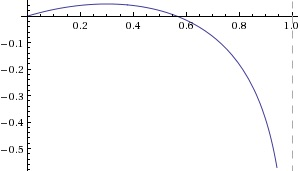
\includegraphics[width=\linewidth]{plotGF}}
      \caption{La función $g(f)$ siempre encuentra un máximo y después tiende a $-\infty$}\label{Fig:Gf}
    \end{minipage}
 \end{figure}
 
 A continuación se presenta un teorema que enumera las ventajas de maximizar $g(f)$, dentro de estas pautas se presentan propiedades básicas que cumplen el criterio de Kelly y dan a entender mejor su función en cada apuesta. La prueba de este teorema se omite en esta tesis, pero se puede revisar en Thorp\cite{thorp1969optimal} para el caso de una simple binomial y para un caso más general se deber revisar Breiman\cite{breiman1961optimal}.
 
\begin{itshape}

\paragraph{Teorema} % (fold)
\label{par:teorema}

\begin{enumerate}

	\item Si $g(f) > 0$, entonces $\lim_{n\to\infty}X_n = \infty$ casi seguro. Es decir, para cada $M$ se tiene que $p(\lim \inf{n\to\infty}X_n >M)=1$.

	\item Si $g(f) < 0$, entonces $\lim_{n\to\infty}X_n = 0$ casi seguro. Es decir, para cada $\varepsilon > 0 $ se tiene que $p(\lim \sup_{n\to\infty}X_n <\varepsilon)=1$.
	
	\item Si $g(f) = 0$, entonces $\lim \sup_{n\to\infty}X_n = \infty$ casi seguro y $\lim \inf_{n\to\infty}X_n = 0$ casi seguro.

	\item Dada una estrategia $\phi^*$ que maximiza $E(\log(X_n))$ y cualquier otra estrategia $\phi$ ``esencialmente diferente'' (No necesariamente una estrategia de apuestas fraccionada fija), entonces $\lim_{n\to\infty}X_n(\phi^*)/X_n(\phi)=\infty$ casi seguro.

	\item El tiempo esperado para que la cantidad de capital actual $X_n$ alcance alguna meta fija $C$ es asintóticamente menor con una estrategia que maximice $E(\log(X_n))$.

	\item Supóngase que el retorno en una unidad apostada en el i-ésimo ensayo es la variable aleatoria $U_i$, además supóngase que la probabilidad de éxito es $p_i$ donde $1/2 < p_i < 1$. Entonces, $E(\log(X_n))$ se maximiza escogiendo en cada ensayo la fracción $f_i^* = p_i -q_i$ que maximiza $E(\log(1+f_iU_i))$.

\end{enumerate}
% paragraph Teorema 1 (end)
\end{itshape}

De la parte 1 de este teorema se muestra que excepto para un número finito de términos, el capital del jugador $X_n$ sobrepasará una cota fija $M$ cuando $f$ se escoge dentro del intervalo $(0,f_c)$. Pero, si $f>f_c$, entonces la parte 2 muestra que la ruina será casi segura. La parte 3 demuestra que si $f=f_c$, entonces $X_n$ (casi seguro) oscilará aleatoriamente entre $0$ y $\infty$. Las partes 4 y 5 establecen que la estrategia de Kelly de maximizar $E(\log(X_n))$ es asintóticamente óptima ya que si se toma una estrategia ``esencialmente diferente'' como aquella tal que la diferencia, $E(\log(X_n^*)) - E(\log(X_n))$, entre la estrategia de Kelly y cualquier otra estrategia crece más rápido que la desviación estándar de $\log(X_n^*) - \log(X_n)$, asegurando $p(\log(X_n^*)-\log(X_n)>0) \to 1$. Finalmente, la parte 6 establece la validez de utilizar el método de Kelly para escoger $f_i*$ en cada uno de los ensayos (aun cuando las probabilidades cambian de un ensayo a otro) con el fin de maximizar $E(\log(X_n))$.

\subsubsection{Ejemplificando Kelly} % (fold)
Retómese la situación descrita al principio de esta sección de un jugador contra un adversario infinitamente rico. Supóngase que el jugador gana la apuesta con una probabilidad $p=0.53$, que su capital inicial es de $X_0$ y que su capital es infinitamente divisible y disponible para apostar. Aplicando el Teorema parte 5, se tiene que $f^* = p-q =0.53-0.47 = 0.06$. Es decir, el jugador debe apostar $6\%$ de su capital para hacerlo crecer $X_n$ a la mayor tasa posible con probabilidad cero de irse a la quiebra. De igual manera, si el jugador continuamente apuesta una fracción más pequeña que el $6\%$, también su capital se irá al infinito, pero la velocidad de crecimiento será menor.

Ahora, si se resuelve numéricamente la ecuación $g(f) = 0.53\log(1+f)+0.47\log(1-f)=0$ se obtiene que $f_c= 0.119712...$. Esto quiere decir que el usuario puede apostar hasta tantito menos del $12\%$ de su capital y como en el caso anterior, su capital se iría al infinito pero a menor escala que con el óptimo. Después del $12\%$, aunque el jugador pudiera ganar dinero a una velocidad mayor que la de la estrategia óptima, al final su capital se irá a cero (casi seguro). 

En cuanto a la tasa de crecimiento, se tienen que $g(f*)= 0.001801$ por lo que después de $n$ apuestas exitosas, su capital crecerá $0.001801n$ veces más dinero que con el que comenzó. De aquí se puede calcular el tiempo esperado de doblar la cantidad de dinero del capital, se tiene que $0.001801n=\log2$. Es decir que después de $n=385$ ensayos se estará doblando la cuenta del jugador.
% paragraph ejemplificando (end)

\subsubsection{Aplicando Kelly a las apuestas de futbol} % (fold)
\label{subsubsection:aplicando_kelly_a_las_apuestas_de_futbol}

El criterio de Kelly se puede extender a las apuestas de futbol. Retómese la situación original, pero ahora considerando que el jugador puede ganar $b$ pesos por cada peso invertido en la apuesta. Además, considérese que el jugador seleccionará sólo apuestas favorables, es decir que sólo apostará cuando la probabilidad de ganar $p>0$ sea ventajosa, i.e. $pb - q > 0$.
De la misma manera se maximiza la siguiente función\footnote{Esta optimización y la fórmula, que a la fecha es tan usada por todos los sitios de apuestas, tuvo su aparición en  Thorp \cite{thorp1969optimal}, aquí mismo se puede encontrar su demostración formal}:
\[g(f) = E\left(log(\frac{X_n}{X_0})\right)=p\log(1+bf)+q\log(1-f)\]
Y se obtiene que:
\[f^* = \frac{bp -q}{b}\]
Esta $f^*$ dicta la fracción del capital que el jugador debe apostar en \textbf{cada} apuesta. Es decir, que la cantidad a apostar depende de dos cosas: Primero, de la probabilidad de éxito de la apuesta. Segundo, del posible retorno de inversión de la apuesta (momio).

\subsubsection{Ejemplo. Kelly en apuestas de futbol}

\emph{Tómese el siguiente partido, Real Madrid vs Juventus. El análisis que se realizó del partido sugiere que la probabilidad de ganar de la Juventus es de $54\%$. Curiosamente, el momio de esta apuesta es $6.75$
¿Cuál es la cantidad de dinero que se debe jugar en esta favorable apuesta?}\linebreak[2]


La solución viene de evaluar $f^*$:
\[f^* = \frac{bp -q}{b} = \frac{(6.75-1)*0.54 - 0.46}{6.75-1} = 0.46\]
Por lo tanto, en este inimaginable escenario, se debe jugar el $46\%$ del capital total en esta apuesta.
\linebreak[2]



Hay tres quejas a considerar sobre Kelly: La primera tiene que ver con el supuesto de ``divisibilidad infinita'', ya que las casas de apuestas usualmente tienen una cantidad mínima para las apuestas y algunas casas tienen todas sus apuestas en función de múltiplos de estos mínimos (o créditos), esto implica que  (casi seguro) siempre se alcanza la ruina. La segunda, va más enfocada a los mercados financieros que implican la posibilidad de pérdidas (``commodity futures'' o ``securities short sales''), en estos casos se puede perder una cierta cantidad de dinero $a$ con probabilidad $q$. Entonces, al resolver, se tiene que la esperanza es igual a $m=bp-aq>0$, $f^*=m/ab >0$; para este caso, se sugiere al lector revisar Thorp y Kassouf \cite{thorp1967beat} y revisar en su detalle la generalización de la formulación y sus detalles. Finalmente, como se vio en los tiempos esperados para duplicar el capital, Kelly es muy lento en el crecimiento del capital al garantizar la ruina con probabilidad $0$; esto hace que en temporadas de futbol (con una cantidad de juegos) el criterio sirva únicamente de guía.

Browne \cite{browne2000can} llama al criterio de Kelly \cite{kelly1956new} como la estrategia óptima de crecimiento, o como la estrategia de utilidad logarítmica. Menciona que es óptima cuando en una variedad de circunstancias la ganancia crece multiplicativamente, únicamente. Hace énfasis que la mayoría de las propiedades de optimalidad son asintóticas en naturaleza (hacia un horizonte infinito), en su trabajo analiza las propiedades de la estrategia de Kelly a corto plazo.


 \section{Proceso para la selección de apuestas}

% Uno de los conceptos más imporantes en la teoría de probabilidad es el del valor esperado de una variable aleatoria\footnote{Retómese el concepto de variable aleatoria más usual, se puede utilizar la definición del capítulo 4 del libro de Ross \cite{ross2006first}, una función $X$ que genera valores aleatorios reales en un espacio muestral completamente definido.}, en palabras del señor Ross \cite{ross2006first} el valor esperado de $X$ se define como un promedio ponderado de los valores posibles que puede tomar $X$; se pondera cada valor con la probabilidad de que $X$ tome ese preciso valor.
%  \begin{itemize}
%
%  	\item Valor esperado de una variable discreta.
%
% 		\[E[X] = \sum_{x:p(x)>0}x p(x)\]
%  	\item Valor esperado de una variable continua.
% 	\[E[X] = \int_{-\infty}^{infty} f(x) dx\]	
 % \end{itemize}
 
 El proceso de la recomendación de apuestas se puede dividir en cinco pasos principales:

 \begin{enumerate}
 	\item \textbf{Determinación de apuestas redituables.} De todas las apuestas de las cinco ligas que haya en la jornada a recomendar, se escogen únicamente aquellas que sean redituables a largo plazo. Independientemente del nivel de riesgo de cada cliente, se generarán recomendaciones únicamente de apuestas que, al analizarlas, tengan ganancias esperadas.
 	\item \textbf{Selección de apuestas de acuerdo al riesgo del cliente.} Las estimaciones de cada partido tienen un intervalo de confianza. Con base en este intervalo y el perfil de riesgo del usuario se seleccionan las apuestas.
 	\item \textbf{Cálculo de la proporción del dinero a invertir por apuesta.} Al conocer la selección de las apuestas, se calcula la proporción de dinero a invertir para cada apuesta, este proceso sigue siendo dependiente de la confianza de la estimación del partido y de la aversión al riesgo del cliente.
 	\item \textbf{Determinación del nivel de reservas.} En este paso se cuenta con un conjunto seleccionado de apuestas y la proporción de dinero que se debe invertir para cada una de ellas. Acorde a su encuesta, se calcula el nivel óptimo de reservas que le permitan al cliente seguir apostando a pesar de que tenga una mala jornada y pierda todas las apuestas.
 	\item \textbf{Recomendación.} Todos estos elementos constituyen en su totalidad la recomendación de la semana que se presenta en el portal al cliente.
 \end{enumerate}
 
Para definir el escenario completo es necesario definir las variables que se utilizan en el proceso, así como las funciones de utilidad que modelan los perfiles de riesgo de los usuarios. Después de estas dos sub-secciones se retomará paso a paso la explicación del proceso de recomendación de apuestas.
 
\subsection{Variables necesarias}
\label{subsec:variables-necesarias}
En este apartado de la tesis se explica cómo se determinan los partidos que se recomiendan a los clientes.
Las variables que se necesitan utilizar son las siguientes:
\begin{enumerate}
	\item \textbf{Probabilidades.} Ya en apartados anteriores se habló de las probabilidades estimadas de que ocurran los tres diferentes resultados de cada encuentro de la jornada (Victoria del local, del visitante y empate). Estas probabilidades son alimentadas a través del portal administrativo.
	
	\item \textbf{Momios.} Los momios que generan las casas de apuestas para cada partido. En la mayoría de los escenarios el usuario escoge usar todos los momios de todos los bookies, en estos casos se tomarán los momios que ofrezcan mejores retornos para cada partido. Estos momios se toman de la información pública de las casas de apuestas.
	
	\item \textbf{Variables de riesgo.} Se tienen tres elementos principales que generan la noción de riesgo en el sistema:
	\begin{itemize}
		\item \textbf{Función de utilidad en selección.} Determina los partidos redituables de la jornada.
		\item \textbf{Función de utilidad del dinero.} Dicta la proporción de dinero a apostar en cada partido.
		\item \textbf{Variable de reserva.} Marca la cantidad de dinero que el cliente debería guardar para siguientes apuestas.
		Estas variables dependen de la encuesta que se le presenta al cliente al crear su cuenta.
	\end{itemize}
	
	\item \textbf{Variable de evolución de ingreso del cliente.} Se define como la cantidad de dinero que tiene el cliente en esta jornada entre la máxima cantidad de dinero que ha tenido. Esta variable genera una noción, en caso de que existan, de la magnitud de las pérdidas que ha tenido el cliente.
\end{enumerate}

\subsection{Funciones de utilidad}
Para modelar el comportamiento de un individuo ante el riesgo, se utilizan funciones de utilidad. Estas funciones representan la utilidad (o beneficio) que un individuo puede obtener por una apuesta. Las funciones más arriesgadas le dan valores mayores valores a las apuestas que que ofrecen las mejores ganancias y las funciones más conservadoras favorecen aquellas apuestas con mayores probabilidades.
En particular, se podría decir de manera intuitiva que el valor obtenido por una función de utilidad para una apuesta en particular es la cantidad de unidades de dinero que el individuo estaría dispuesto a invertir en esa apuesta.
El siguiente listado presenta las funciones que se utilizan actualmente en el sistema.
\begin{enumerate}
		\item \textbf{Polinomial - lineal:} 
		\[f_1(\alpha, p, m) = \left(\frac{p}{1-p} \right)^\frac{1}{1-\alpha}(m-1)^\frac{\alpha}{1-\alpha}\]
Parámetro $\alpha$ que va de cero a uno. Es una de las familias más volátiles en cuanto al riesgo, para valores cercanos a uno del parámetro tiende a ser muy arriesgada, casi sin diversificar, y para valores cercanos a cero tiende a ser muy conservadora y suele diversificar mucho más en las apuestas.

		\item \textbf{Polinomial - cuadrática:} 
		\[f_2(\alpha, p, m) = \left(\frac{p}{1-p} \right)^\frac{1}{2-\alpha}(m-1)^\frac{\alpha}{2-\alpha}\]
Esta familia de funciones es muy parecida a la anterior, también tiene un parámetro $\alpha$ entre cero y uno, sólo que en este caso no es tan extremista como en el caso anterior.
		
		\item \textbf{Exponencial - lineal:} 
		\[f_3(\alpha, p, m) = \left(\frac{1}{m-1} \right)ln\left(\frac{\alpha p(m-1)}{1-p}\right)\]
Esta familia de funciones tiene un parámetro $\alpha$ que es mayor a uno. Es una familia de funciones conservadoras que suelen proteger muy bien adelantándose a semanas malas, a costo que en semanas buenas no logran tan buenos beneficios.
		
		\item \textbf{Lineal - exponencial:} 
		\[f_4(\alpha, p, m) = ln\left(\frac{p(m-1)}{1-p}\right) + ln(\alpha)\]
Esta familia de funciones tiene un parámetro $\alpha$ que es mayor a uno. Es una familia de funciones que le gusta fuertemente diversificar, aparte tiende a favorecer un poco aquellas apuestas más riesgosas.

		\item \textbf{Logarítmica - polinomial:} 
		\[f_5(\alpha, p) = \left(\frac{p}{1-p}\right)^\frac{1}{\alpha}\]
Parámetro $\alpha$ mayor a uno. Es una familia de funciones muy conservadora ya que toma valores sin considerar los momios del mercado, al tomar en cuenta solamente las probabilidades de los partidos tiende a ser más estable en el tiempo.

		\item \textbf{Tangente - lineal:} 
		\[f_6(\alpha, p, m) = \frac{1}{m-1}\sqrt{\frac{pm - (1-\alpha)p - \alpha}{1-p}}\]
		Parámetro $\alpha$ entre cero y uno. Esta familia es la más conservadora de la lista, busca tener las menores pérdidas posibles y protege las inversiones cada semana.
\end{enumerate}

Estas seis funciones son las que utiliza Egobets para modelar la aversión al riesgo de sus clientes. Cuando ellos llenan la encuesta del perfil, realmente están seleccionando una de estas funciones.


\subsection{Paso 1 - Determinación de apuestas redituables}
\label{sec:paso-1}


Para seguir la explicación de los pasos del proceso se tomará un ejemplo práctico y las transformaciones que sufre durante el proceso. Al empezar las recomendaciones de una jornada se tiene un conjunto de datos muy parecido al que se da en el ejemplo. Tómese la tabla~\ref{momios-y-probas} como base del ejemplo. En esta tabla se presentan momios de alguna casa de apuesta (usualmente los mejores del mercado) para diez partidos distintos, cada uno cuenta con los momios para los tres tipos de apuestas: victoria del Local ($m_L$), empate ($m_E$) y victoria del visitante ($m_V$). Además se muestran las probabilidades estimadas por Egobets de los tres posibles resultados del encuentro: victoria del local ($\hat{p_L}$), empate ($\hat{p_L}$) y victoria del visitante ($\hat{p_L}$).

\begin{table}[ht]
\centering
\resizebox{\textwidth}{!}{%
\begin{tabular}{|c|ccc|ccc|}
\toprule
{\textbf{Partido}}                 & $\mathbf{m_L}$ & $\mathbf{m_E}$ & $\mathbf{m_V}$ & $\mathbf{\hat{p_L}}$ & $\mathbf{\hat{p_E}}$ & $\mathbf{\hat{p_V}}$ \\ \midrule
A & 2.6  & 3.2  & 2.75  & 0.31  & 0.23  & 0.46  \\ 
B & 2.1  & 3.3  & 3.5   & 0.37  & 0.3   & 0.32  \\ 
C & 1.11 & 8.5  & 21    & 0.84  & 0.1   & 0.04  \\ 
D & 4.5  & 3.75 & 1.72  & 0.29  & 0.27  & 0.45  \\ 
E & 2    & 3.4  & 3.75  & 0.37  & 0.31  & 0.31  \\ 
F & 1.53 & 4    & 6     & 0.61  & 0.17  & 0.21  \\ 
G & 2.1  & 3.25 & 3.6   & 0.51  & 0.24  & 0.25  \\ 
H & 1.9  & 3.4  & 4     & 0.42  & 0.29  & 0.29  \\ 
I & 1.8  & 3.5  & 4.5   & 0.46  & 0.29  & 0.25  \\ 
J & 1.9  & 3.4  & 4     & 0.5   & 0.26  & 0.23  \\ \bottomrule
\end{tabular}
}
\caption{Diez partidos con sus respectivos momios y las probabilidades estimadas por Egobets}
\label{momios-y-probas}
\end{table}

Para concretar el ejemplo, se fijarán las siguientes funciones y variables.
\begin{itemize}
	\item \textbf{Función de selección.} Tómese la \emph{Polinomial - lineal} $f_1$ con parámetro $\alpha = 0.4$.
	\item \textbf{Función de utilidad del dinero.} Úsese la \emph{Exponencial - lineal} con parámetro $\alpha = 3$
	\item \textbf{Variable de reserva.} Será $v_R = 15$.
	\item \textbf{Variable de ingreso.} Será $v_I = 0.80$.
\end{itemize}
	

Ahora para proceder al primer paso, defínase el valor esperado de una apuesta como la multiplicación de la probabilidad de que suceda el resultado por el momio que se tiene para esa apuesta. 
Con el ejemplo bien definido se procede a filtrar las apuestas con el primer paso. De manera intuitiva, se podría enunciar que el valor esperado de una apuesta corresponde a la cantidad de unidades de dinero que se obtienen por cada unidad de dinero invertida\footnote{Recuérdese que esta cantidad incluye la cantidad de dinero invertida en la apuesta. También recuérdese que la ganancia solamente se obtiene si se gana la apuesta.}

Entonces, el primer paso consiste en utilizar para las recomendaciones, sólo las apuestas con ganancias a largo plazo; las otras apuestas tendrán un valor esperado no positivo, es decir, no garantizan más que pérdidas a largo plazo. Más aun, se usarán solo las apuestas que garanticen un valor esperado mayor a $1.025$, esta restricción tiene dos ventajas, la primera es que las probabilidades que se usan son estimaciones por lo que ese $2.5\%$ funciona como protección para no caer en valores esperados negativos y la segunda es que si el rendimiento es tan pequeño toma mucho tiempo para un cliente ir acumulando ganancias. 

\begin{table}[ht]
\centering
\resizebox{\textwidth}{!}{%
\begin{tabular}{|c|ccc|ccc|ccc|c|}
\toprule
Partido & $\mathbf{m_L}$ & $\mathbf{m_E}$ & $\mathbf{m_V}$ & $\mathbf{\hat{p_L}}$ & $\mathbf{\hat{p_E}}$ & $\mathbf{\hat{p_V}}$ & $\mathbf{m_L\cdot\hat{p_V}}$ & $\mathbf{m_E\cdot\hat{p_E}}$ & $\mathbf{m_V\cdot\hat{p_V}}$ & \textbf{Apuesta} \\ \midrule
A & 2.6 & 3.2 & 2.75 & 0.31 & 0.23 & 0.46 & 0.81 & 0.74 & \textbf{1.27} & Visitante \\
B & 2.1 & 3.3 & 3.5 & 0.37 & 0.3 & 0.32 & 0.78 & 0.99 & \textbf{1.12} & Visitante \\
C & 1.11 & 8.5 & 21 & 0.84 & 0.1 & 0.04 & 0.93 & 0.85 & 0.84 & Ninguna \\
D & 4.5 & 3.75 & 1.72 & 0.29 & 0.27 & 0.45 & \textbf{1.31} & 1.01 & 0.77 & Local \\
E & 2 & 3.4 & 3.75 & 0.37 & 0.31 & 0.31 & 0.74 & \textbf{1.05} & \textbf{1.16} & Empate/Visitante \\
F & 1.53 & 4 & 6 & 0.61 & 0.17 & 0.21 & 0.93 & 0.68 & \textbf{1.26} & Visitante \\
G & 2.1 & 3.25 & 3.6 & 0.51 & 0.24 & 0.25 & \textbf{1.07} & 0.78 & 0.90 & Local \\
H & 1.9 & 3.4 & 4 & 0.42 & 0.29 & 0.29 & 0.80 & 0.99 & \textbf{1.16} & Visitante \\
I & 1.8 & 3.5 & 4.5 & 0.46 & 0.29 & 0.25 & 0.83 & 1.02 & \textbf{1.13} & Visitante \\
J & 1.9 & 3.4 & 4 & 0.5 & 0.26 & 0.23 & 0.95 & 0.88 & 0.92 & Ninguna\\ \bottomrule
\end{tabular}
}
\caption{Escogiendo apuestas que vale la pena realizar}
\label{redituables}
\end{table}

Obsérvese en la tabla~\ref{redituables} como en negritas se han señalado las posibles apuestas a realizar. De las treinta posibles apuestas, ahora sólo quedan 9 redituables. Hay dos partidos el `C' y el `J' que no ameritan apuesta alguna. Y el partido `E', por ejemplo, tiene dos posibles apuestas redituables.

\subsection{Paso 2 - Selección de apuestas}
\label{sec:paso-2}


Para determinar el portafolio de apuestas basta con calcular el valor de la función de utilidad de selección y se deben tomar aquellas ``$n$'' apuestas que tengan los mayores valores (Donde ``$n$'' es el número de apuestas a recomendar).
Ver tabla~\ref{seleccion}

\begin{table}[ht]
\centering
\resizebox{\textwidth}{!}{%
\begin{tabular}{|c|c|c|c|c|}
\toprule
\textbf{Partido} & \textbf{Apuesta} & \textbf{Momio} & $\mathbf{\hat{p}}$ & $\mathbf{f_1(\alpha, p, m)}$ \\ \midrule
A & Visitante & 2.75 & 0.46 & \textbf{1.07} \\
B & Visitante & 3.5 & 0.32 & 0.53 \\
D & Local & 4.5 & 0.29 & 0.49 \\
E & Empate & 3.4 & 0.31 & 0.48 \\
E & Visitante & 3.75 & 0.31 & 0.53 \\
F & Visitante & 6 & 0.21 & 0.31 \\
G & Local & 2.1 & 0.51 & \textbf{1.12} \\
H & Visitante & 4 & 0.29 & 0.48 \\
I & Visitante & 4.5 & 0.25 & 0.36\\ \bottomrule
\end{tabular}
}
\caption{Escogiendo apuestas que vale la pena realizar}
\label{seleccion}
\end{table}

\subsection{Paso 3 - Calcular cuanto dinero a cada apuesta}
\label{sec:paso-3}

Una vez determinado el portafolio de apuestas hace falta determinar la cantidad de dinero que se invertirá en éste. Esta sección y la próxima resolverán tal problema.
 Se empieza por determinar cuál es la proporción de dinero que se invertirá en cada apuesta. La solución es sencilla, ya se determinó en secciones anteriores que el valor definido por una función de utilidad puede ser comparado con la cantidad de unidades de dinero que una persona estaría dispuesta a invertir en una apuesta en particular. El único problema con este enfoque es que tales cantidades no se encuentran en ninguna escala (es decir, dólares, pesos, etc).Se hace lo siguiente: para cada apuesta se calcula el valor de su función de utilidad del dinero y después lo dividimos entre la suma de todos estos valores para todas las apuestas que se van a tomar, de esta forma se tiene los números como porcentajes.
 Regresando al ejemplo: (En este caso la función de utilidad del dinero era Exponencial-Lineal con parámetro 3)
Ver tabla~\ref{proporcion}

\begin{table}[ht]
\centering
\resizebox{\textwidth}{!}{%
\begin{tabular}{|c|c|c|c|c|}
\toprule
\textbf{Partido} & \textbf{Apuesta} & \textbf{Momio} & $\mathbf{\hat{p}}$ & $\mathbf{f_3(\alpha, p, m)}$ \\ \midrule
A & Visitante & 2.75 & 0.46 & 0.23 \\
G & Local & 2.1 & 0.51 & 0.35 \\ \bottomrule
\end{tabular}
}
\caption{Calculando la proporción del dinero que se debe invertir en estas apuestas}
\label{proporcion}
\end{table}


Los valores suman a 0.59, cuando se divide cada valor por 0.59 resulta: De la cantidad a apostar, se debe de apostar $40 \%$ en el partido A a visitante y $60 \%$ en el partido G a local.


\subsection{Paso 4 - Determinar nivel de reservas}
\label{sec:paso-4}

%[COMENTARIO]ESto no creo que vaya aquí, estas propiedades deberían estar definidas en otro lugar
% El sistema de reservas, en pocas palabras, tiene como intención proteger el dinero de los clientes en el corto plazo, de tal forma que si una semana resulta en pérdidas, éstas no vayan a afectar la tendencia a largo plazo de sus ingresos totales. Las ventajas de usar un sistema de reservas son las siguientes: primero, como ya se dijo, proteger el dinero del cliente en el corto plazo cuando haya pérdidas, en segundo lugar, permite al cliente mantener el mismo nivel de apuestas cada semana, y tercero, permite darle una estructura de fondo de inversión a las apuestas y así poder aprovechar el potencial interés compuesto que resulte de apostar. En contraste, las desventajas son: en cada semana se decide apostar menos dinero y por lo tanto las ganancias son menores en el corto plazo, además al ser una estrategia de largo plazo, los clientes que deseén incurrir en mayores riesgos no usarán este sistema de reservas.
%
% Un sistema de reservas da más flexibilidad de la que inicialmente se podría pensar, estas son algunas de las propiedades que serían deseables en un sistema de esta forma:
% \begin{enumerate}
% \item Se tenga la seguridad de que con alta probabilidad el apostador nunca va a perder todo su dinero.
%
% \item Que en aquellas semanas que son mas riesgosas se apueste menos dinero, para protegerse del riesgo.
%
% \item Que en aquellas semanas donde se pueden tener muchas ganancias se apueste una mayor cantidad de dinero, para tratar de aprovechar situaciones ventajosas.
%
% \item Que cuando se tengan pérdidas se apueste una mayor cantidad de dinero para tratar de recuperar el nivel anterior de ganancias lo más pronto posible.
% \end{enumerate}
% Como se ve, este sistema tiene la propiedad de ser dinámico y que depende tanto de las circunstancias de las apuestas como también del historial de ganancias del cliente.

Determinar el nivel de reservas es un algoritmo que depende del historial de ganancias del cliente así como de las circunstancias de las apuestas que se le presentan al cliente. A continuación se explica paso a paso como determinar el nivel de reservas.

\begin{enumerate}
	\item \textbf{Calcular la cantidad de partidos a los que se apuesta.}
	
	
Defínase $j$,$k$ como la cantidad de partidos a apostar y el número de apuestas a tomar, respectivamente.
En este pasó bastará con calcular $j$. Sin embargo, es importante notar que hay veces en las que puede haber más de una apuesta sugerida para un mismo partido, i.e. $k>j$. En estos casos se deberá ser cuidadoso de no contar doble los partidos que ya tengan apuestas.

	% Sea $k$ el número de a
	% \lstset{language=Pascal}
	% \begin{lstlisting}[frame=single]
	% begin
	% 	apuestas := 0;
	% 	aux2 := 0;
	% 	for i:= 1 to K do
	% 	begin
	% 		if (proporcion(i) >= 1/k) then
	% 			aux1 := aux1 + 1;
	% 		else
	% 			aux2 := aux2 + proporcion(i);
	% 	end;
	% 	partidosApostables := aux1 + round((k)aux2);
	% end.
	% \end{lstlisting}
	%
	\item \textbf{Calcular el valor esperado y varianza del portafolio de apuesta.}
	
	
	Sean $m_i$, $p_i$ y $prop_i$; el momio, la probabilidad y la proporción de dinero a apostar del partido $i$ respectivamente. Entonces el valor esperado de la apuesta sería:
	\[\mu = \sum_{i=1}^{k}{(prop_i)(m_i)(p_i)}\]
	Y el riesgo o varianza del portafolio de apuestas se calcula así:
	\[\sigma = \sqrt{\sum_{i=1}^{k}{(prop_i))^2(m_i)^2(p_i)(1-p_i)}}\]
	
	
	\item \textbf{Actualizar el riesgo del portafolio.}
	
	
	Sea $\rho$ el parámetro de reserva un número entero entre $10$ y $25$ dependiendo de la encuesta del cliente. Se actualiza el riesgo del portafolio al multiplicarlo por un escalar proveniente de la raíz cuadrada del cociente de la cantidad de partidos $j$ entre el parámetro de reserva $\rho$.
	\[\sigma = \left(\sqrt{\frac{j}{\rho}}\right)\sigma\]
	

	\item \textbf{Calcular probabilidad de riesgo.}
	
	Sea $X$ la variable de evolución del ingreso del cliente (Esta variable es completamente dependiente de las historia de perdidas y ganancias del cliente). Y sea $p_\sigma$ la probabilidad de riesgo y se calcula de la siguiente manera:
	\[p_\sigma = \frac{1}{1.749615}(I_1 + I_2) - 1.06 + X\]
	Donde $I_1$ es
	\[I_1 = 0.2925 +1.3772\mu - 1.127\rho\]
	e $I_2$ equivale a
	\[I_2 = \frac{3.11}{\mu}(1 + 0.792\sigma - \mu)((-0.567345 + 1.3772\mu -1.17\sigma)\mu X)^{0.123}\]
	
	
	\item \textbf{Calcular variable proxy.}
	
	 Sea $proxy$ la variable auxiliar que tome en cuenta la probabilidad de riesgo en el cálculo.
	 \[proxy = 0.2925 + 1.3772\mu -1.127\sigma - 0.9975p_\sigma\]
	
	\item \textbf{Calcular el nivel de reserva.}
	
	Finalmente, defínase $c_A$ cómo el porcentaje a apostar del ingreso total. El nivel de reserva será uno menos esta proporción.
	
	\begin{equation*}
	    c_A = \begin{cases}
	               0.05            & \text{si } \frac{j(proxy)}{\rho} < 0.05\\
	               1               & \text{si } \frac{j(proxy)}{\rho} >1\\
	              	\frac{j(proxy)}{\rho} & \text{en otro caso}
	           \end{cases}
	\end{equation*}
	
	$C_A$ representa, en porcentaje, la cantidad de dinero que se le recomendará al cliente que apueste en esa semana para el portafolio de apuestas en cuestión.
	
	\textbf{Calculando el nivel de reserva en el ejemplo.}
	
	Primero que nada es importante recordar cuanto valían las distintas variables y establecer los valores necesarios para el ejemplo.
	\begin{itemize}
		\item $k = 2$ (Cantidad apuestas a realizar)
		\item $\rho = 15$ (Parámetro de reserva en función de las preferencias del cliente)
		\item $X = 0.80$ (Evolución del ingreso del cliente)		
	\end{itemize}
	Ahora se procederá a calcular el nivel de reservas.
	\begin{enumerate}
		\item Se obtiene $j = 2$ (Cantidad de partidos en los que se apuesta)
		\item Se calcula el valor esperado 
		\[\mu = (0.4)(2.75)(0.46) + (0.6)(2.1)(0.51) = 1.1486\] 
		y el riesgo del portafolio 
		\[\sigma = \sqrt{(0.4)^2(2.75)^2(0.46)(0.54)+(0.6)^2(2.1)^2(0.51)(0.49)} = 0.835\]
		\item Se actualiza el riesgo $\sigma = \left(\sqrt{\frac{2}{15}}\right)0.835 = 0.3$
		\item Se calcula la probabilidad de riesgo
		\[I_1 = 0.2925 +1.3772(1.1486) - 1.127(0.3) = 1.53\]
		\[I_2 = \frac{3.11}{1.1486}(1 + 0.792(0.3) - \mu)((-0.567345 + 1.3772(1.1486)\]
		\[-1.17(0.3))(1.1486)(0.8))^{0.123} = 0.2272\]
		Entonces
		\[p_\sigma = \frac{1}{1.749615}(1.53 + 0.2272) - 1.06 + 0.8 = 0.74\]
		
		\item Se calcula la variable auxiliar $proxy = 0.2925 + 1.3772(1.1486) -1.127(0.3) - 0.9975(0.74) = 0.81$
		
		\item La cantidad a apostar es entonces es igual a $c_A = \frac{2(0.81)}{15} = 0.108$
		Por lo tanto, con esta aversión al riesgo y con base en el portafolio de apuestas de la tabla~\ref{proporcion}.
		
		\textbf{El nivel de reserva para esta recomendación es del} $\mathbf{89.2\%}$.
	\end{enumerate}
\end{enumerate}

\subsection{Paso 5 - Presentando la recomendación}
\label{sec:paso-5}
Ahora, con todos los pasos cumplidos lo único restante es poner las cifras juntas. Se toma la proporción calculada en~\ref{sec:paso-3} y se multiplica por la cantidad a apostar obtenida en~\ref{sec:paso-4}.
Más aún, si el usuario proporciona la cantidad de dinero que tiene disponible, las recomendaciones se pueden expresar en moneda.

Finalmente si para el ejemplo planteado en~\ref{sec:paso-1} se conoce que el usuario tiene $\$10'000.00$ para apostar, la recomendación de apuesta quedaría de la siguiente manera:
\begin{enumerate}
	\item Apueste $\$432$ pesos ($4.32\%$) en el partido A a favor del equipo visitante.
	\item Apueste $\$648$ pesos ($8.48\%$) en el partido G a favor del equipo local.
\end{enumerate}


